%  Registers.tex
%  Document created by seblovett on seblovett-Ubuntu
%  Date created: Tue 01 Apr 2014 20:10:32 BST
%  <+Last Edited: Fri 04 Apr 2014 12:29:48 BST by hl13g10 on octopus +>

\section{Registers}\label{sect:regs}

%\todo[inline]{Design}
The allocation in the instruction set allows for up to 16 general purpose registers. 
In the program, discussed in section \ref{sect:prog}, only 11 registers are used. 
Six are used to store the constants, two for the initial vector, two for the result and a temporary register.
To save RAM, only the required registers are implemented.
This still requires a four bit address and attempting to address the registers above the valid range would result in undefined behaviour.

The registers were implemented using the Synchronous RAM.
This, at the expense of performance, utilised the on chip SRAM blocks. 
The design was parametrised to allow the data and address width and number of registers to be easily changed. 

%\todo[inline]{Explain Test Bench}

\subsection{Testbench}

A task is used to do a basic test.
The code for this task is seen in listing \ref{lstregtask}.
A random byte of data, and a random register are chosen. 
The data is then written to the register. 
The input data is changed to check that the data on the output is stored in memory and assertions are used to verify. 
The data is checked to persist after the write enable signal is inactive. 
If an assertion fails, a global error counter is incremented.

This task is then done a large amount of times to check all registers. 
Figure \ref{fig:regsim} shows the output waveform of the simulation. 
The error count is zero at the end of the simulation showing that the module is functioning correctly.




\lstinputlisting[style=sverilog,firstline=33, lastline=51,caption={Register task for writing and reading to the register.},label=lstregtask]{../Implementation/registers_stim.sv}
%\todo[inline]{Simulation Results}

\begin{figure}
\includegraphics[width=\textwidth,height=\textheight]{Figures/registerssim.eps}
\caption{Waveform simulation for register testbench}
\label{fig:regsim}
\end{figure}

\subsection{Synthesis}
%\todo[inline]{Synthesis}

The synthesised logic of the register module is shown in \ref{fig:registersynth}.
This is virtually identical to the Program ROM module, seen in figure \ref{fig:ramsynth} apart from the write address and data are inputs, rather than hardwired constants.
This utilises the internal SRAM of the FPGA. 

\begin{figure}
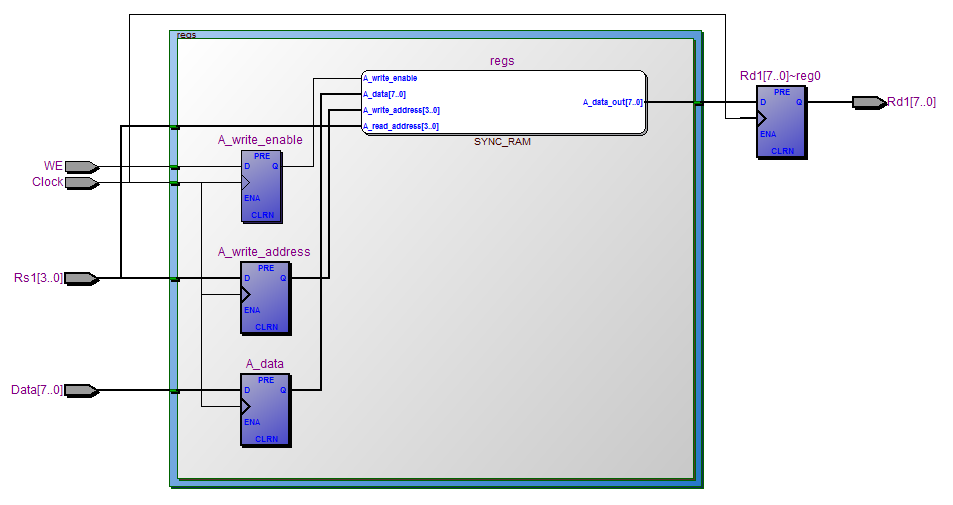
\includegraphics[width=\textwidth]{Figures/registersynth.png}
\caption{Synthesis of the register module}
\label{fig:registersynth}
\end{figure}
